\subsection{Código Ótimo}

\begin{frame}[allowframebreaks]
  \frametitle{Em busca do código ótimo}
  \begin{itemize}
  \item Código de Prefixo $\leftrightarrow$ desigualdade de Kraft.
  \item Precisamos apenas encontrar os comprimentos $l_i$ que satisfazem Kraft e então
	criar um código de prefixo com estes comprimentos.
  \item Objetivo: minimizar o comprimento esperado do código.
	\begin{equation}
	L(C) = \sum_i p_i l_i
	\end{equation}
  \item Problema de otimização com restrição:
	\begin{equation}
	\min_{ \{ l_{1:m} \} \in \mathbb{Z}_{+}^m  } \sum_i p_i l_i \quad \text{sujeito a} \sum_i D^{-l_i} \leq 1 
	\end{equation}
  \item Problema de programação em inteiros que é um problema NP-difícil, provavelmente não será
	solucionado de forma eficiente (a menos que $P=NP$).
  \item Relaxar a condição sobre $l_i$ ser inteiro. Considerar o Lagrangiano e encontrar os comprimentos ótimos.
	\begin{equation}
	l_i^\ast = -\log_D p_i
	\end{equation}
  \item Entropia é o comprimento esperado mínimo: $L \geq H_D (X)$.
  \item $L-H$ é uma medida do quão distante estamos do ótimo.
	\begin{equation}
	L-H = D(p \mid \mid r) + \log_D 1/c , 
	\end{equation}
	onde $c = \sum_i D^{-l_i}$ e $r_i = \frac{D^{-l_i}}{\sum_j D^{-l_j}}$.
  \item Para construir um código, encontramos a distribuição $D$-ádica mais próxima (KL) de $p$ e construímos
	um código seguindo a proposição inversa de Kraft.
  \item Código de Shannon: $l_i = \lceil \log_D 1/p_i \rceil$. Estes comprimentos satisfazem Kraft. Logo existe
	um código de prefixo com estes comprimentos. Teremos $H_D(X) \leq L \leq H_D(X) + 1$.
	Teremos que a eficiência $\rightarrow 1$ quando $H(X) \rightarrow \infty$, mas quando $H(X) \rightarrow 0$
	teremos que a eficiência $\rightarrow 0$. Por exemplo, quando $D=2$ teremos eficiência máxima de 50\%.
	\begin{equation}
	0 \leq \text{eficiência} \triangleq \frac{H_D (X)}{E l(X)} \leq 1
	\end{equation}
  \item Podemos melhorar a eficiência codificado em blocos.
	\begin{equation}
	H(X_1, \ldots, X_n) \leq E l(X_{1:n}) \leq H(X_1, \ldots, X_n) + 1
	\end{equation}
  \item Codificar com a distribuição errada $q$ implica em:
	\begin{equation}
	H(p) + D(p \mid \mid q) \leq E_p l(X) \leq H(p) + D(p \mid\mid q) + 1
	\end{equation}
	onde utilizamos $l(x) = \lceil \log 1/q(x) \rceil$ e a distribuição subjacente é $p$.
  \end{itemize}
\end{frame}


\subsection{Código de Shannon é ótimo?}
\begin{frame}[allowframebreaks]
  \frametitle{Código de Shannon é ótimo?}
  \begin{example}
  \begin{itemize}
  \item Suponha $\mathcal{X} = \{0,1\}$ com $p(X = 0) = 10^{-1000} = 1 - p(X=1)$.
  \item Comprimentos de Shannon serão: 
	\begin{itemize}
	\item $l(0) = \lceil \log_2 10^{-1000} \rceil = 3322$ bits.
	\item $l(1) = \lceil \log_2 (1 - 10^{-1000}) \rceil = 1$ bit.
	\end{itemize}
	Para o símbolo $0$ estamos utilizando 3321 bits a mais do que o necessário.
  \item De forma geral, pode acontecer que $\lceil \log_D p_i \rceil$ é maior do que o necessário.
  \item O código de Shannon não é um código de prefixo com comprimentos inteiros ótimo.
  \end{itemize}
  \end{example}
\end{frame}


\subsection{Código de Guloso}
\begin{frame}[allowframebreaks]
  \frametitle{Código de Huffman}
  \begin{itemize}
  \item \textbf{Procedimento} para encontrar o menor código de prefixo. (Por ser um procedimento
	é difícil analisar matematicamente).
  \item Objetivo: dado $p(x)$, queremos encontrar o menor código de prefixo.
  \end{itemize}
\end{frame}

\begin{frame}[allowframebreaks]
  \frametitle{Método Guloso}
  \begin{itemize}
  \item Abordagem gulosa: começar pelo topo e dividir as palavras potenciais em probabilidades iguais
	(i.e., realizar perguntas com entropia máxima).
	\begin{itemize}
	\item Esta abordagem é similar ao jogo das 20 perguntas. Temos um conjunto de objetos
		$\mathbf{S} = \{1, 2, 3, \ldots, m\}$ que ocorre com frequência proporcional aos
		pesos não negativos $(w_1, w_2, \ldots, w_m)$.
	\item Queremos determinar qual o objeto realizando o menor número de perguntas possível.
	\item Cada pergunta será da forma `$X \in \mathbf{A}$?' onde $\mathbf{A} \subseteq \mathbf{S}$.
	\item Supondo $\mathbf{S} = \{x_1, x_2, x_3, x_4, x_5 \}$.
		\begin{figure}[h!]
		\centering
		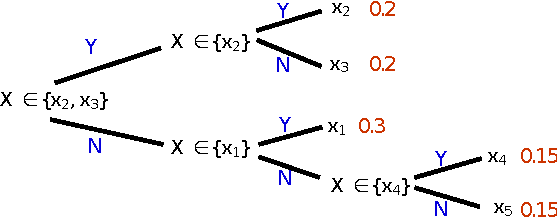
\includegraphics[width=0.65\textwidth]{images/synq.pdf}
		\caption{Exemplo \citep{bilmes2013}.}
		\label{fig:synq}
		\end{figure}
	\item Charles Sanders Peirce, 1901
		\begin{quote}
		Thus twenty skillful hypotheses will ascertain what two
		hundred thousand stupid ones might fail to do. The secret
		of the business lies in the caution which breaks a
		hypothesis up into its smallest logical components, and
		only risks one of them at a time.
		\end{quote}
	\end{itemize}
  \item Método Guloso: na próxima etapa fazer aquilo que parece melhor naquele instante. 
  \item Considere a distribuição
	\begin{tabular}{c|c|c|c|c|c|c|c}
		  & a    & b    & c    & d    & e    & f    & g \\ \hline
		p & 0.01 & 0.24 & 0.05 & 0.20 & 0.47 & 0.01 & 0.02
	\end{tabular}
  \item A pergunta que parece melhor é aquela que infere mais sobre a distribuição, reduz a entropia residual sobre $X$,
	será então a pergunta $Y_1$ com maior entropia. Teremos
	\begin{eqnarray}
	H(X|Y_1) &=& H(X,Y_1) - H(Y_1) \\
		 &=& H(X) - H(Y_1)
	\end{eqnarray}
	onde utilizamos o fato de que $Y_1$ é uma função de $X$, e assim $H(X,Y_1) = H(X)$.
  \item Escolhemos a pergunta $Y_1$ com maior informação mútua com $X$.
	\begin{equation}
	I(Y_1 ; X) = H(X) - H(X|Y_1) = H(Y_1)
	\end{equation}
  \item As perguntas são da forma `$X \in \mathbf{A}$?' onde $\mathbf{A} \subseteq \mathbf{S}$.
	Desta forma, escolher uma pergunta do tipo sim-não é o mesmo que escolher o conjunto $\mathbf{A}$.
  \item Considere a seguinte partição $\{a,b,c,d,e,f,g\} = \{a,b,c,d\} \cup \{e,f,g\}$. A pergunta
	`$X \in \{e,f,g\}$?' terá entropia máxima, pois $p(X \in \{a,b,c,d\}) = p(X \in \{e,f,g\}) = 0.5$.
  \item A pergunta corresponde à v.a. $Y_1 = \mathbf{1}_{\{X \in \{e,f,g\}\}}$, então
	$H(Y_1) = 1$, o que seria considerado uma boa pergunta.
  \item A próxima pergunta depende do resultado da pergunta anterior.
  \item Se $Y_1 = 0$ ($\equiv X \in \{a,b,c,d\}$) poderemos fazer a partição $\{a,b,c,d\} = \{a,b\} \cup \{c,d\}$,
	já que $p(\{a,b\}) = p(\{c,d\}) = 1/4$. Ou seja, $p(X \in \{a,b\} \mid X \in \{a,b,c,d\}) = 1/2$ e
	$p(X \in \{c,d\} \mid X \in \{a,b,c,d\}) = 1/2$.
  \item Esta pergunta corresponde à v.a. $Y_2 = \mathbf{1}_{\{X \in \{c,d\}\}}$. Teremos $H(Y_2 \mid Y_1 = 0) = 1$, e assim
	esta seria considerada uma boa pergunta.
  \item Para $Y_1 = 1$ precisaremos particionar $\{e,f,g\}$
	\begin{tabular}{c|c|c|c}
		 & I & II & III \\ \hline
	partição & $(\{e\},\{f,g\})$ & $(\{e,f\},\{g\})$ & $(\{e,g\},\{f\})$ \\ \hline
	prob	 & $(0.47, 0.03)$ & $(0.48, 0.02)$ & $(0.49, 0.01)$ \\ \hline
	$H(Y_2 \mid Y_1 = 1)$ & $0.3274$ & $0.2423$ & $0.1414$
	\end{tabular}
	A partição I é aquela que fornece a pergunta com maior entropia.
  \item Temos
	\begin{eqnarray}
	H(X \mid Y_2, Y_1) &=& H(X,Y_2 \mid Y_1) - H(Y_2 \mid Y_1) \\
			&=& H(X \mid Y_1) - H(Y_2 \mid Y_1) \\
			&=& H(X) - H(Y_2 \mid Y_1) - H(Y_1)
	\end{eqnarray}
  \item Abordagem gulosa: a cada passo escolhemos o que nos parece melhor, as escolhas futuras terão que lidar
	com as possibilidades que restaram devido às escolhas passadas.
  \item partições
	\begin{scriptsize}
	\hspace*{-1cm}
	\begin{tabular}{c|c|c|c}
	conjunto	  & partição & probabilidades & entropia condicional \\ \hline
	$\{a,b,c,d,e,f,g\}$ 	& $\{a,b,c,d\}$ , $\{e,f,g\}$ 	& $(0.5, 0.5)$ 		& $H(Y_1) = 1$ \\ \hline
	$\{a,b,c,d\}$ 		& $\{a,b\}$, $\{c,d\}$		& $(0.25, 0.25)$ 	& $H(Y_2 \mid Y_1 = 0) = 1$ \\ \hline
	$\{e,f,g\}$		& $\{e\}$, $\{f,g\}$ 		& $(0.47, 0.03)$ 	& $H(Y_2 \mid Y_1 = 1) = 0.3274$ \\ \hline
	$\{a,b\}$		& $\{a\}$, $\{b\}$		& $(0.01, 0.24)$	& $H(Y_3 \mid Y_2 = 0, Y_1 = 0) = 0.2423$ \\ \hline
	$\{c,d\}$		& $\{c\}$, $\{d\}$		& $(0.05, 0.20)$	& $H(Y_3 \mid Y_2 = 1, Y_1 = 0) = 0.7219$ \\ \hline
	$\{e\}$			& $\{e\}$ 			& $(0.47)$		& $H(Y_3 \mid Y_2 = 0, Y_1 = 1) = 0$ \\ \hline
	$\{f,g\}$		& $\{f\}$ ,$\{g\}$		& $(0.01, 0.02)$ 	& $H(Y_3 \mid Y_2 = 1, Y_1 = 1) = 0.9183$ 
	\end{tabular}
	\end{scriptsize}
  \item Observe que $H(X) = H(Y_1, Y_2, Y_3) = 1.9323$ e lembre que
	\begin{eqnarray}
	H(Y_1, Y_2, Y_3) &=& H(Y_1) + H(Y_2 \mid Y_1) + H(Y_3 \mid Y_1 , Y_2) \\
			&=& H(Y_1) + \sum_{i \in \{0,1\}} H(Y_2 \mid Y_1 = i) p(Y_1 = i)  \nonumber \\
			&&	+ \sum_{i,j \in \{0,1\}} H(Y_3 \mid Y_1 = i, Y_2 = j) p(Y_1 = i, Y_2 = j) \nonumber
	\end{eqnarray}


  \framebreak
  \item Árvore obtida através do método guloso

        \begin{tabular}{c|c|c|c|c|c|c|c}
                  & a    & b    & c    & d    & e    & f    & g \\ \hline
                p & 0.01 & 0.24 & 0.05 & 0.20 & 0.47 & 0.01 & 0.02
        \end{tabular}


        \hvFloat[floatPos=htb,capPos=right,capVPos=bottom,objectPos=c]{figure}{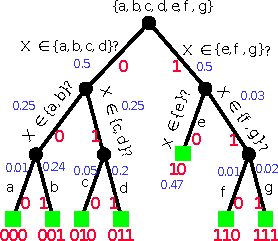
\includegraphics[width=0.3\textwidth]{images/greedytree.pdf}}
	{Árvore obtida através do método guloso \citep{bilmes2013}.}{fig:greedytree}
         %       \begin{figure}[h!]
         %       \centering
         %       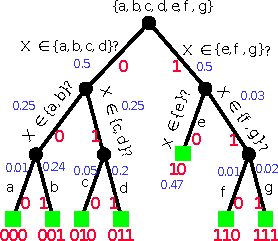
\includegraphics[width=0.4\textwidth]{images/greedytree.pdf}
         %       \label{fig:greedytree}
         %       \end{figure}

	\begin{itemize}
	\item comprimento esperado do código $E l = 2.53$
	\item entropia $H=1.9323$
	\item eficiência $H/E l = 0.7638$
	\end{itemize}

  \item Comparando o método guloso com o método de Huffman.
        \hvFloat[floatPos=htb,capPos=right,capVPos=bottom,objectPos=c]{figure}{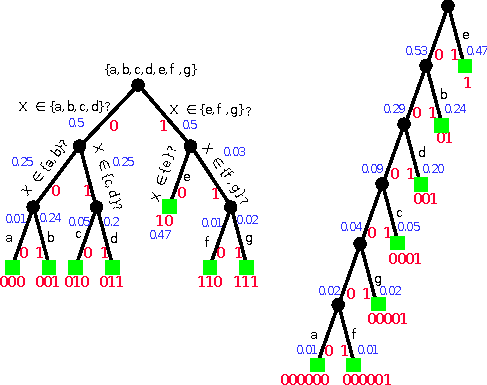
\includegraphics[width=0.4\textwidth]{images/greedyvshuffman.pdf}}
	{Guloso vs Huffman \citep{bilmes2013}.}{fig:greedyvshuffman}
         %       \begin{figure}[h!]
         %       \centering
         %       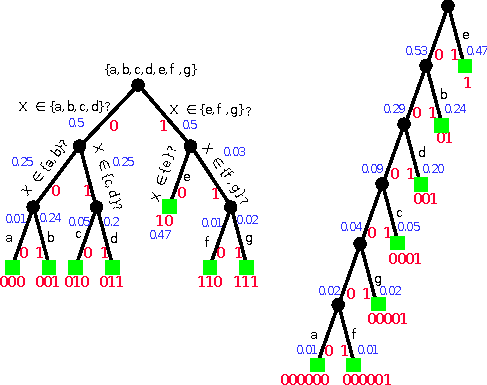
\includegraphics[width=0.55\textwidth]{images/greedyvshuffman.pdf}
         %       \label{fig:greedyvshuffman}
         %       \end{figure}
	\begin{itemize}
        \item comprimento esperado do código $E l_{\text{huffman}} = 1.97$
	\item eficiência $H/E l_{\text{huffman}} = 0.9809$
	\item logo, o método guloso não é ótimo
        \end{itemize}

  \end{itemize}
\end{frame}


\subsection{Código de Huffman}
\begin{frame}[allowframebreaks]
  \frametitle{Código de Huffman}
  \begin{itemize}
  \item Procedimento
	\begin{enumerate}
	\item Selecione os dois símbolos menos prováveis no alfabeto.
	\item Ambos terão associados as palavras mais longas e se diferirão no último bit.
	\item Combine estes dois símbolos em um símbolo auxiliar com probabilidade igual à soma das 
		probabilidades dos dois símbolos. Adicione o símbolo auxiliar e remova os dois símbolos previamente selecionados.
		Repita os passos.
	\end{enumerate}
  \item Estratégia \textit{bottom-up}.
  \item A estratégia é similar para $D > 2$. Neste caso poderá ser necessário utilizar símbolos fictícios no alfabeto.
  \item O comprimento das palavras em um código Huffman não são sempre $\leq \lceil \log 1/p_i \rceil$ (comprimento de Shannon).
  \end{itemize}

  \begin{example}
  \begin{itemize}
  \item $\mathcal{X} = \{1,2,3,4,5\}$ com probabilidades $(1/4, 1/4, 1/5, 3/20, 3/20)$.

         \begin{figure}[h!]
         \centering
         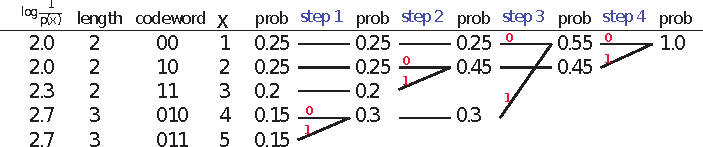
\includegraphics[width=0.95\textwidth]{images/ex-huffman01.pdf}
         \label{fig:ex-huffman01}
         \end{figure}

  \item $E l = 2.3$ bits e $H=2.2855$ bits.
  \item Algumas palavras são maiores e outras menores que $l^\ast(x) = I(X) = \log 1/p(x)$.
  \end{itemize}
  \end{example}

  \framebreak
  \begin{example}
  Considere $\mathcal{X}$ com probabilidades $(\frac{1}{3}, \frac{1}{3}, \frac{1}{4}, \frac{1}{12})$.
  \begin{itemize}
  \item Entropia $H=1.8554$ bits.
  \item Comprimentos de Huffman são: $L_{h1} = (2,2,2,2)$ ou $L_{h2} = (1,2,3,3)$.
  \item Comprimentos de Shannon $\lceil \log 1/p_i \rceil$ são $L_s = (2,2,2,4)$ e assim $E L_s = 2.1557 > 2$. 
	Note que $l_s(x_3) < l_{h2} (x_3)$, mas na média o comprimento esperado de Huffman é menor.
  \end{itemize}
  \end{example} 

\end{frame}


\begin{frame}[allowframebreaks]
  \frametitle{Código de Huffman é ótimo}
  O código de Huffman é ótimo, i.e., $\sum_i p_i l_i$ é mínimo para comprimentos inteiros.

  Para mostrar iremos fazer:
  \begin{enumerate} 
  \item Lemma: alguns códigos ótimos possuem certas propriedades ($\exists$ código ótimo com estas propriedades).
  \item Dado um código $C_m$ para $m$ símbolos, com tais propriedades, podemos criar um código mais simples satisfazendo o lemma e que será
	mais fácil otimizar.
  \item Ao final da recurção chegaremos ao caso simples de dois símbolos em que a otimização é trivial.
  \end{enumerate}

  \framebreak
  \begin{lemma}
  Para toda distribuição, $\exists$ um código instantâneo ótimo (i.e., com comprimento esperado mínimo)
  satisfazendo simultâneamente:
  \begin{enumerate}
  \item Se $p_j > p_k$ então $l_j \leq l_k$ (i.e., o símbolo mais provável não possui palavra com maior comprimento).
  \item As duas maiores palavras possuem o mesmo comprimento.
  \item As duas maiores palavras diferem apenas no último bit e correspondem aos dois símbolos menos prováveis.
  \end{enumerate}
  \end{lemma}

  \framebreak
  \begin{proof}
  \begin{itemize}
  \item Suponha que $C_m$ seja um código ótimo (então $L(C_m)$ é mínimo) e escolha $j,k$ de forma tal que $p_j > p_k$.
	Precisamos mostrar que $\exists$ um código com $l_j \leq l_k$.
  \item Considere o código $C_m'$ com a troca das palavras $j$ e $k$, ou seja,
	\begin{equation}
	l_j' = l_k \quad \text{e} \quad l_k' = l_j
	\end{equation}
	o que só pode tornar o código maior, então $L(C_m') \geq L(C_m)$.
  \end{itemize}
  \proofbreak
  \begin{itemize}
  \item Realizando a troca, como $L(C_m)$ é mínimo, teremos
	\begin{eqnarray}
	0 &\leq& L(C_m') - L(C_m) = \sum_i p_i l_i' - \sum_i p_i l_i \nonumber \\
		&=& p_j l_j' + p_k l_k' - p_j l_j - p_k l_k = p_j l_k + p_k l_j - p_j l_j - p_k l_k \nonumber \\
		&=& p_j (l_k - l_j) - p_k (l_k - l_j) \nonumber \\
		&=& \underbrace{(p_j - p_k)}_{>0}  (l_k - l_j)
	\end{eqnarray}
  \item Devemos ter então $(l_k - l_j) \geq 0$, ou seja, $l_k \geq l_j$ quando $p_j > p_k$, satisfazendo assim a propriedade 1.
  \end{itemize}
  \proofbreak
  \begin{itemize}
  \item Na verdade, esta propriedade é verdadeira para todos códigos ótimos.
  \item Propriedade 2: as palavras mais longas possuem o mesmo comprimento.
  \item Se as duas palavras maiores não possuem o mesmo comprimento, podemos apagar o último bit da palavra mais longa.
	Desta forma manteremos a propriedade de prefixo, já que a palavra mais longa é a única com o seu dado comprimento e não
	existe um prefixo dela que seja uma outra palavra.
         \begin{figure}[h!]
         \centering
         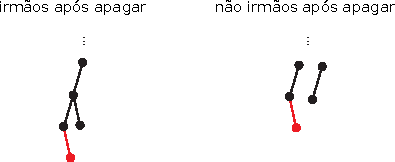
\includegraphics[width=0.355555\textwidth]{images/lemmahuffman.pdf}
         \label{fig:lemmahuffman}
         \end{figure}
  \end{itemize}
  \proofbreak
  \begin{itemize}
  \item Desta forma reduzimos o comprimento esperado. Concluímos que um código ótimo deve possuir as duas
	palavras mais longas com o mesmo comprimento.
  \item Propriedade 3: as duas palavras mais longas diferem apenas no último bit e correspondem aos símbolos menos prováveis.
  \item Devido à propriedade 1 ($p_k < p_j \Rightarrow l_k \geq l_j$), se $p_k$ é a menor probabilidade, então ela deve
	possuir associada uma palavra de comprimento que não seja menor do que qualquer outra $j$ com $p_j > p_k$. 
	De forma similar, se $p_k$ é a segunda menor probabilidade, a palavra associada deve possuir comprimento que não seja
	menor do que qualquer outro símbolo mais provável.
  \end{itemize}
  \proofbreak
  \begin{itemize}
  \item As duas palavras mais longas possuem o mesmo comprimento (propriedade 2) e correspondem aos dois símbolos menos prováveis.
  \item Se as duas maiores palavras não são irmãs, podemos trocá-las. Isto é, se $p_1 \geq p_2 \geq \ldots \geq p_m$, então
	fazemos a transposição ilustrada:
         \begin{figure}[h!]
         \centering
         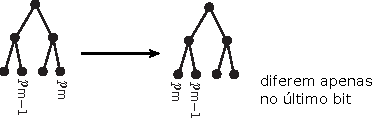
\includegraphics[width=0.4\textwidth]{images/lemmahuffman2.pdf}
         \label{fig:lemmahuffman2}
         \end{figure}
  \item Isto não altera o comprimento esperado $L = \sum_i p_i l_i$.
  \end{itemize}
  \end{proof}

  \begin{itemize}
  \item Então, se $p_1 \geq p_2 \geq \ldots \geq p_m$, existe um código ótimo com $l_1 \leq l_2 \leq \ldots l_{m-1} = l_m$
	e no qual $C(x_{m-1})$ e $C(x_m)$ diferem apenas no último bit.
  \item Vamos mostrar que Huffman é ótimo através da operação de criar um novo código no qual a otimização é mais simples.
	Este processo é repetido até que a otimização seja trivial.
  \item Assuma um código $C_m$ (não necessariamente ótimo) que satisfaz as propriedades anteriores.
	$C_m$ terá as seguintes palavras de código $\{w_i\}_{i=1}^m$.
  \item Huffman transforma $C_m$ em $C_{m-1}$ com palavras de código $\{w_i'\}_{i=1}^{m-1}$.
  \item Índices $m$ e $m-1$ terão menor probabilidade e palavras maiores.
	\begin{tabular}{ccc}
	$C_m$ & comprimento & prob. do símbolo \\ \hline
	$w_1$ & $l_1$ & $p_1$ \\
	$w_2$ & $l_2$ & $p_2$ \\
	$\vdots$ & $\vdots$ & $\vdots$ \\
	$w_{m-2}$ & $l_{m-2}$ & $p_{m-2}$ \\
	$w_{m-1}$ & $l_{m-1}$ & $p_{m-1}$ \\
	$w_{m}$ & $l_{m}$ & $p_{m}$ \\
	\end{tabular}
  \end{itemize}
  \framebreak
  \begin{itemize} 
  \item Huffman realiza a seguinte operação para ir de $C_m$ para $C_{m-1}$:
 	\begin{tabular}{cccccc}
	\scriptsize{prob. símb.} & $C_{m-1}$ & \scriptsize{comp.} $m-1$ & \scriptsize{rel. código} & \scriptsize{rel. comp.} & \scriptsize{prob. símb.} \\ \hline
	$p_1$	& $w_1'$	& $l_1'$	& $w_1 = w_1'$ 	& $l_1 = l_1'$ 	& $p_1$ \\
	$p_2$   & $w_2'$        & $l_2'$        & $w_2 = w_2'$  & $l_2 = l_2'$  & $p_2$ \\
	$\vdots$ & $\vdots$ & $\vdots$ & $\vdots$ & $\vdots$ & $\vdots$ \\
	$p_{m-2}$   & $w_{m-2}'$        & $l_{m-2}'$        & $w_{m-2} = w_{m-2}'$  & $l_{m-2} = l_{m-2}'$  & $p_{m-2}$ \\
	$p_{m-1} + p_m$   & $w_{m-1}'$        & $l_{m-1}'$        & $w_{m-1} = w_{m-1}' 0$  & $l_{m-1} = l_{m-1}'+1$  & $p_{m-1}$ \\
		& 	& 	& $w_{m} = w_{m-1}' 1$ & $l_m = l_{m-1}'+1$ & $p_m$
	\end{tabular}
  \item $w_i$ e $l_i$ são as palavras e comprimento das palavras do código $C_m$ e $w_i'$ e $l_i'$ do código $C_{m-1}$.
  \item As palavras e comprimentos em Huffman são definidos recursivamente. Huffman define uma relação entre palavras 
	(e consequentemente comprimentos) ao dar um passo de um código para outro mais simples.
  \item Teremos o seguinte:
	\begin{eqnarray}
	L(C_m) &=& \sum_i p_i l_i \nonumber \\
		&=& \sum_{i=1}^{m-2} p_i l_i' + p_{m-1} (l_{m-1}' + 1) + p_m (l_{m-1}' + 1) \nonumber \\
		&=& \sum_{i=1}^{m-2} p_i l_i' + (p_{m-1} + p_m) l_{m-1}' + p_{m-1} + p_m \nonumber \\
		&=& \sum_{i=1}^{m-1} p_i' l_i'+ p_{m-1} + p_m \nonumber \\
		&=& L(C_{m-1}) + \underbrace{p_{m-1} + p_m}_{\text{não involve comprimentos}}
	\end{eqnarray}
  \item Desta forma, reduzimos o número de variáveis que iremos otimizar (de $m$ para $m-1$).
  \item Procedimento de Huffman implica em
	\begin{eqnarray}
	\min_{l_{1:m}} L(C_m) &=& \text{const.} + \min_{l_{1:m-1}} L(C_{m-1}) = \ldots \nonumber \\
			&=& \text{const.} + \min_{l_{1:2}} L(C_{2})
	\end{eqnarray}
	onde em cada passo são preservadas as propriedades.
  \item Ao reduzir para o caso com dois comprimentos, teremos a solução óbvia, um bit para cada símbolo, e assim
	podemos refazer o caminho de volta e construir o código.
  \item Em cada passo garantimos que estaremos obtendo a solução ótima, e assim o código criado pelo algoritmo de Huffman
	será ótimo.
  \end{itemize}

  \begin{theorem}
  O procedimento de codificação de Huffman cria um código com comprimentos inteiros ótimo.
  \end{theorem}

  \begin{itemize}
  \item Cada símbolo terá associado uma palavra formada por um número inteiro de bits.
  \item Para distribuições que não são $D$-ádicas, poderemos utilizar até um bit extra por símbolo, na média.
  \item A codificação de Huffman tem a seguinte propriedade:
	\begin{equation}
	H(X) \leq L(C_{\text{Huffman}}) \leq H(X) + 1
	\end{equation}
  \item A codificação de Huffman em blocos tem a propriedade:
	\begin{equation}
        H(X_{1:n}) \leq L(C_{\text{Huffman em blocos}}) \leq H(X_{1:n}) + 1
        \end{equation}
  \item Podemos obter melhor resultado se codificarmos em bloco. Neste caso precisaremos calcular $p(x_{1:n})$.
  \item Se o alfabeto é de tamanho $\vert \mathcal{X} \vert$, precisaremos de uma tabela de tamanho $\vert \mathcal{X} \vert^n$
	para armazenar todas as probabilidades.
  \item É difícil estimar $p(x_{1:n})$ de forma acurada. Muitas das possíveis \textit{strings} não ocorrerão.
	Será necessário utilizar técnicas de suavização (\textit{smoothing}), como por exemplo Good-Turing \textit{Smoothing}.
  \item Existe também a latência introduzida pelos blocos (será necessário aguardar uma sequência de símbolos formar um bloco
	para poder codificar). Além disso a codificação em blocos demandará maiores recursos computacionais.
  \item Apesar da otimalidade do código de Huffman, duas grandes dificuldades ainda interpõem à sua aplicação:
      1) o desconhecimento da real estatítica da fonte subjacente e 2) opernado em bloso, o crescimento da complexidade do algoritmo 
      com o tamanho do bloco.
  \end{itemize}
\end{frame}

